\documentclass[11pt,a4paper]{article}

% --- Paquetes Principales ---
\usepackage[utf8]{inputenc}
\usepackage[spanish,es-tabla]{babel}
\usepackage{amsmath,amssymb,amsfonts}
\usepackage{graphicx}
\usepackage{geometry}
\usepackage{booktabs}
\usepackage{hyperref}
\usepackage{listings}
\usepackage{xcolor}
\usepackage{subcaption}
\usepackage{float}
\usepackage{microtype}
\usepackage{titlesec}
\usepackage{fancyhdr}

% --- Configuración de Márgenes ---
\geometry{
    top=2.5cm,
    bottom=2.5cm,
    left=2.5cm,
    right=2.5cm
}

% --- Configuración de Enlaces ---
\hypersetup{
    colorlinks=true,
    linkcolor=blue!70!black,
    citecolor=blue!70!black,
    urlcolor=blue!70!black
}

% --- Configuración de Código Fuente (listings) ---
\definecolor{codegreen}{rgb}{0,0.6,0}
\definecolor{codegray}{rgb}{0.5,0.5,0.5}
\definecolor{codepurple}{rgb}{0.58,0,0.82}
\definecolor{backcolour}{rgb}{0.97,0.97,0.97}

\lstdefinestyle{mystyle}{
    backgroundcolor=\color{backcolour},   
    commentstyle=\color{codegreen},
    keywordstyle=\color{blue}\bfseries,
    numberstyle=\tiny\color{codegray},
    stringstyle=\color{codepurple},
    basicstyle=\ttfamily\footnotesize,
    breakatwhitespace=false,         
    breaklines=true,                 
    captionpos=b,                    
    keepspaces=true,                 
    numbers=left,                    
    numbersep=5pt,                  
    showspaces=false,                
    showstringspaces=false,
    showtabs=false,                  
    tabsize=2,
    frame=single,
    rulecolor=\color{gray!30}
}
\lstset{style=mystyle}

% --- Encabezados y Pies de Página ---
\pagestyle{fancy}
\fancyhf{}
\rhead{Proyecto Fashion Peaks}
\lhead{Cuantificación Espectrométrica con CNN}
\cfoot{\thepage}

% =========================================================================
% TÍTULO Y AUTORES
% =========================================================================
\title{
    \vspace{-1.5cm}
    \textbf{\Large INFORME TÉCNICO Y CIENTÍFICO} \\[0.3cm]
    \textbf{\huge Proyecto Fashion Peaks} \\[0.4cm]
    \large Cuantificación de Fotopicos de Cesio-137 en Espectrometría Gamma \\
    mediante Redes Neuronales Convolucionales: Diagnóstico, Decisiones de Diseño y Modelado Comparativo
}
\author{
    \textbf{Luana} \\
    \small Proyecto de Investigación en Inteligencia Artificial Aplicada a la Espectrometría Nuclear \\
    \small Cátedra / Tutor: Prof. Edgardo Bonzi
}
\date{Octubre 2026}

\begin{document}

\maketitle

\begin{abstract}
En el presente trabajo se aborda la determinación automatizada del área de fotopicos de decaimiento radiactivo de Cesio-137 ($^{137}\text{Cs}$, $661.66\text{ keV}$) en espectros gamma provenientes de sedimentos lacustres, utilizando técnicas de visión computacional y redes neuronales convolucionales 2D (\textit{Convolutional Neural Networks}, CNN). Partiendo de los desarrollos iniciales propuestos en el proyecto \textit{Fashion Peaks}, se diagnosticó un fallo sistemático de colapso predictivo en el modelo de clasificación categórica original en el intervalo de áreas intermedias y altas ($9.250$ a $17.250$ unidades), donde las inferencias convergían erróneamente hacia la clase $16.250$. 

Para resolver esta limitación, se implementó una serie de innovaciones metodológicas y arquitecturales: (1) representación espacial continua mediante sombreado de área bajo la curva (\textit{area fill}), (2) reformulación del aprendizaje hacia una \textbf{Regresión Continua de Área} con función de pérdida de Huber (\textit{Huber Loss}), (3) partición rigurosa de datos en entrenamiento (70\%), validación (15\%) y prueba ciega independiente (15\%), y (4) normalización numérica de etiquetas. La evaluación experimental sobre 300 muestras de prueba nunca vistas demostró una resolución contundente del problema: el coeficiente de determinación alcanzó un $R^2 = 0.9955$ ($99.55\%$), el Error Absoluto Medio global se redujo a $97.83$ unidades ($< 0.5\%$ del rango total de $20.000$), y el error en la región crítica se redujo en un \textbf{43\%} (de $777.78$ a $444.23$ unidades), alcanzando un error relativo medio de apenas el $3.81\%$. Se detallan todas las justificaciones teóricas, el funcionamiento pormenorizado del código y los resultados comparativos.
\end{abstract}

\tableofcontents
\newpage

% =========================================================================
% SECCIÓN 1: INTRODUCCIÓN Y CONTEXTO FÍSICO
% =========================================================================
\section{Contexto Físico y Motivación del Proyecto}

\subsection{El Isótopo Cesio-137 y su Importancia Ambiental}
El Cesio-137 ($^{137}\text{Cs}$) es un radioisótopo antropogénico con un período de semidesintegración de aproximadamente $30.08$ años. Su presencia en el medio ambiente proviene fundamentalmente de los ensayos de armamento nuclear en la atmósfera efectuados a mediados del siglo XX (principalmente entre 1954 y 1963) y de accidentes en reactores nucleares (como Chernóbil en 1986). 

Al depositarse sobre la superficie terrestre mediante precipitación húmeda y seca, el $^{137}\text{Cs}$ se fija con notable afinidad a las partículas arcillosas y a la materia orgánica del suelo. Posteriormente, los procesos de erosión hídrica transportan estos sedimentos hacia las cuencas y lagos, acumulándose en estratos cronológicos en el fondo lacustre. Por este motivo, la cuantificación de los perfiles de concentración de $^{137}\text{Cs}$ en testigos de sedimentos lacustres es una herramienta geocronológica fundamental para la datación de sedimentos y el estudio de tasas históricas de erosión y sedimentación.

\subsection{Detección y Espectrometría de Rayos Gamma}
El $^{137}\text{Cs}$ decae por emisión beta ($\beta^-$) a un estado metaestable del Bario-137m ($^{137\text{m}}\text{Ba}$), el cual se desexcita emitiendo un fotón gamma característico de energía monoenergética:
\begin{equation}
E_\gamma = 661.657 \text{ keV}
\end{equation}

Para detectar estas emisiones se emplean detectores de germanio hiperpuro (HPGe) refrigerados a la temperatura del nitrógeno líquido ($77\text{ K}$). Las señales eléctricas producidas por los pulsos ionizantes son amplificadas y digitalizadas en un analizador multicanal (MCA), generando un espectro discreto de intensidad (cuentas) en función de canales de energía (bins).

En dicho espectro, la presencia de Cesio-137 se manifiesta como un pico gaussiano (fotopico) situado a $661.66\text{ keV}$, superpuesto a un fondo continuo y picos naturales (provenientes de series de uranio, torio, y potasio-40). \textbf{El área neta bajo dicho fotopico es directamente proporcional a la actividad radiactiva de la muestra.}

\subsection{La Dificultad del Procesamiento Clásico y la Idea ``Fashion Peaks''}
El análisis clásico exige un ajuste analítico manual (típicamente ajuste gaussiano no lineal con sustracción de línea base Compton). Cuando se dispone de grandes volúmenes de muestras (cientos o miles de espectros), el procesamiento manual resulta sumamente tedioso, lento y dependiente del criterio subjetivo del analista.

Inspirado en el célebre conjunto de datos \textit{Fashion-MNIST} de visión computacional, el proyecto \textbf{Fashion Peaks} propone transformar el problema espectrométrico unidimensional en una tarea de visión artificial: convertir una ventana estrecha de energía en torno a los $661\text{ keV}$ en una imagen de dimensiones reducidas ($32 \times 64$ píxeles) y entrenar una Red Neuronal Convolucional (CNN) 2D para que extraiga los patrones espaciales y cuantifique el área de forma instantánea y reproducible.

% =========================================================================
% SECCIÓN 2: DIAGNÓSTICO DEL TRABAJO INICIAL Y PROBLEMÁTICA
% =========================================================================
\section{Diagnóstico del Trabajo Inicial y Problemática Identificada}

\subsection{El Enfoque Inicial por Clasificación Categórica}
En la etapa inicial del proyecto formulada por el profesor Edgardo Bonzi (documentada en el archivo \texttt{FashioN\_Peaks\_readme.pdf}), el cálculo del área se abordó como un problema de \textbf{clasificación discreta en 41 clases}. El área continua (escalada por un factor de 1000) variaba entre $0$ y $20.000$ unidades. El espacio continuo fue particionado en intervalos fijos de $500$ unidades, asignando como etiqueta el punto medio del intervalo:
\begin{equation}
\text{Clase}(A) = \left\lfloor \frac{A - 1}{500} \right\rfloor \cdot 500 + 250
\end{equation}
Así, valores entre $0$ y $500$ recibían la etiqueta $250$, valores entre $501$ y $1.000$ recibían $750$, y así sucesivamente hasta $20.250$.

La red neuronal utilizada fue \texttt{SpectraCNN}, una arquitectura convolucional sencilla con tres capas de convolución y dos capas densas conectadas a una capa final de activación lineal con función de pérdida de entropía cruzada (\texttt{CrossEntropyLoss}).

\subsection{El Problema del Colapso en el Rango Intermedio-Alto}
Al examinar la matriz de confusión generada por el profesor (véase Figura~\ref{fig:matriz_original}), se descubrió una anomalía crítica:
\begin{quote}
\textit{``De ella se desprende que la región de las áreas que van desde el valor de 9250 al 17250, la CNN tiende a clasificar erróneamente estas áreas dentro de la clase 16250. Por lo que se deberá trabajar para mejorar esta parte de clasificación.''} (README original, pág. 6).
\end{quote}

\begin{figure}[H]
    \centering
    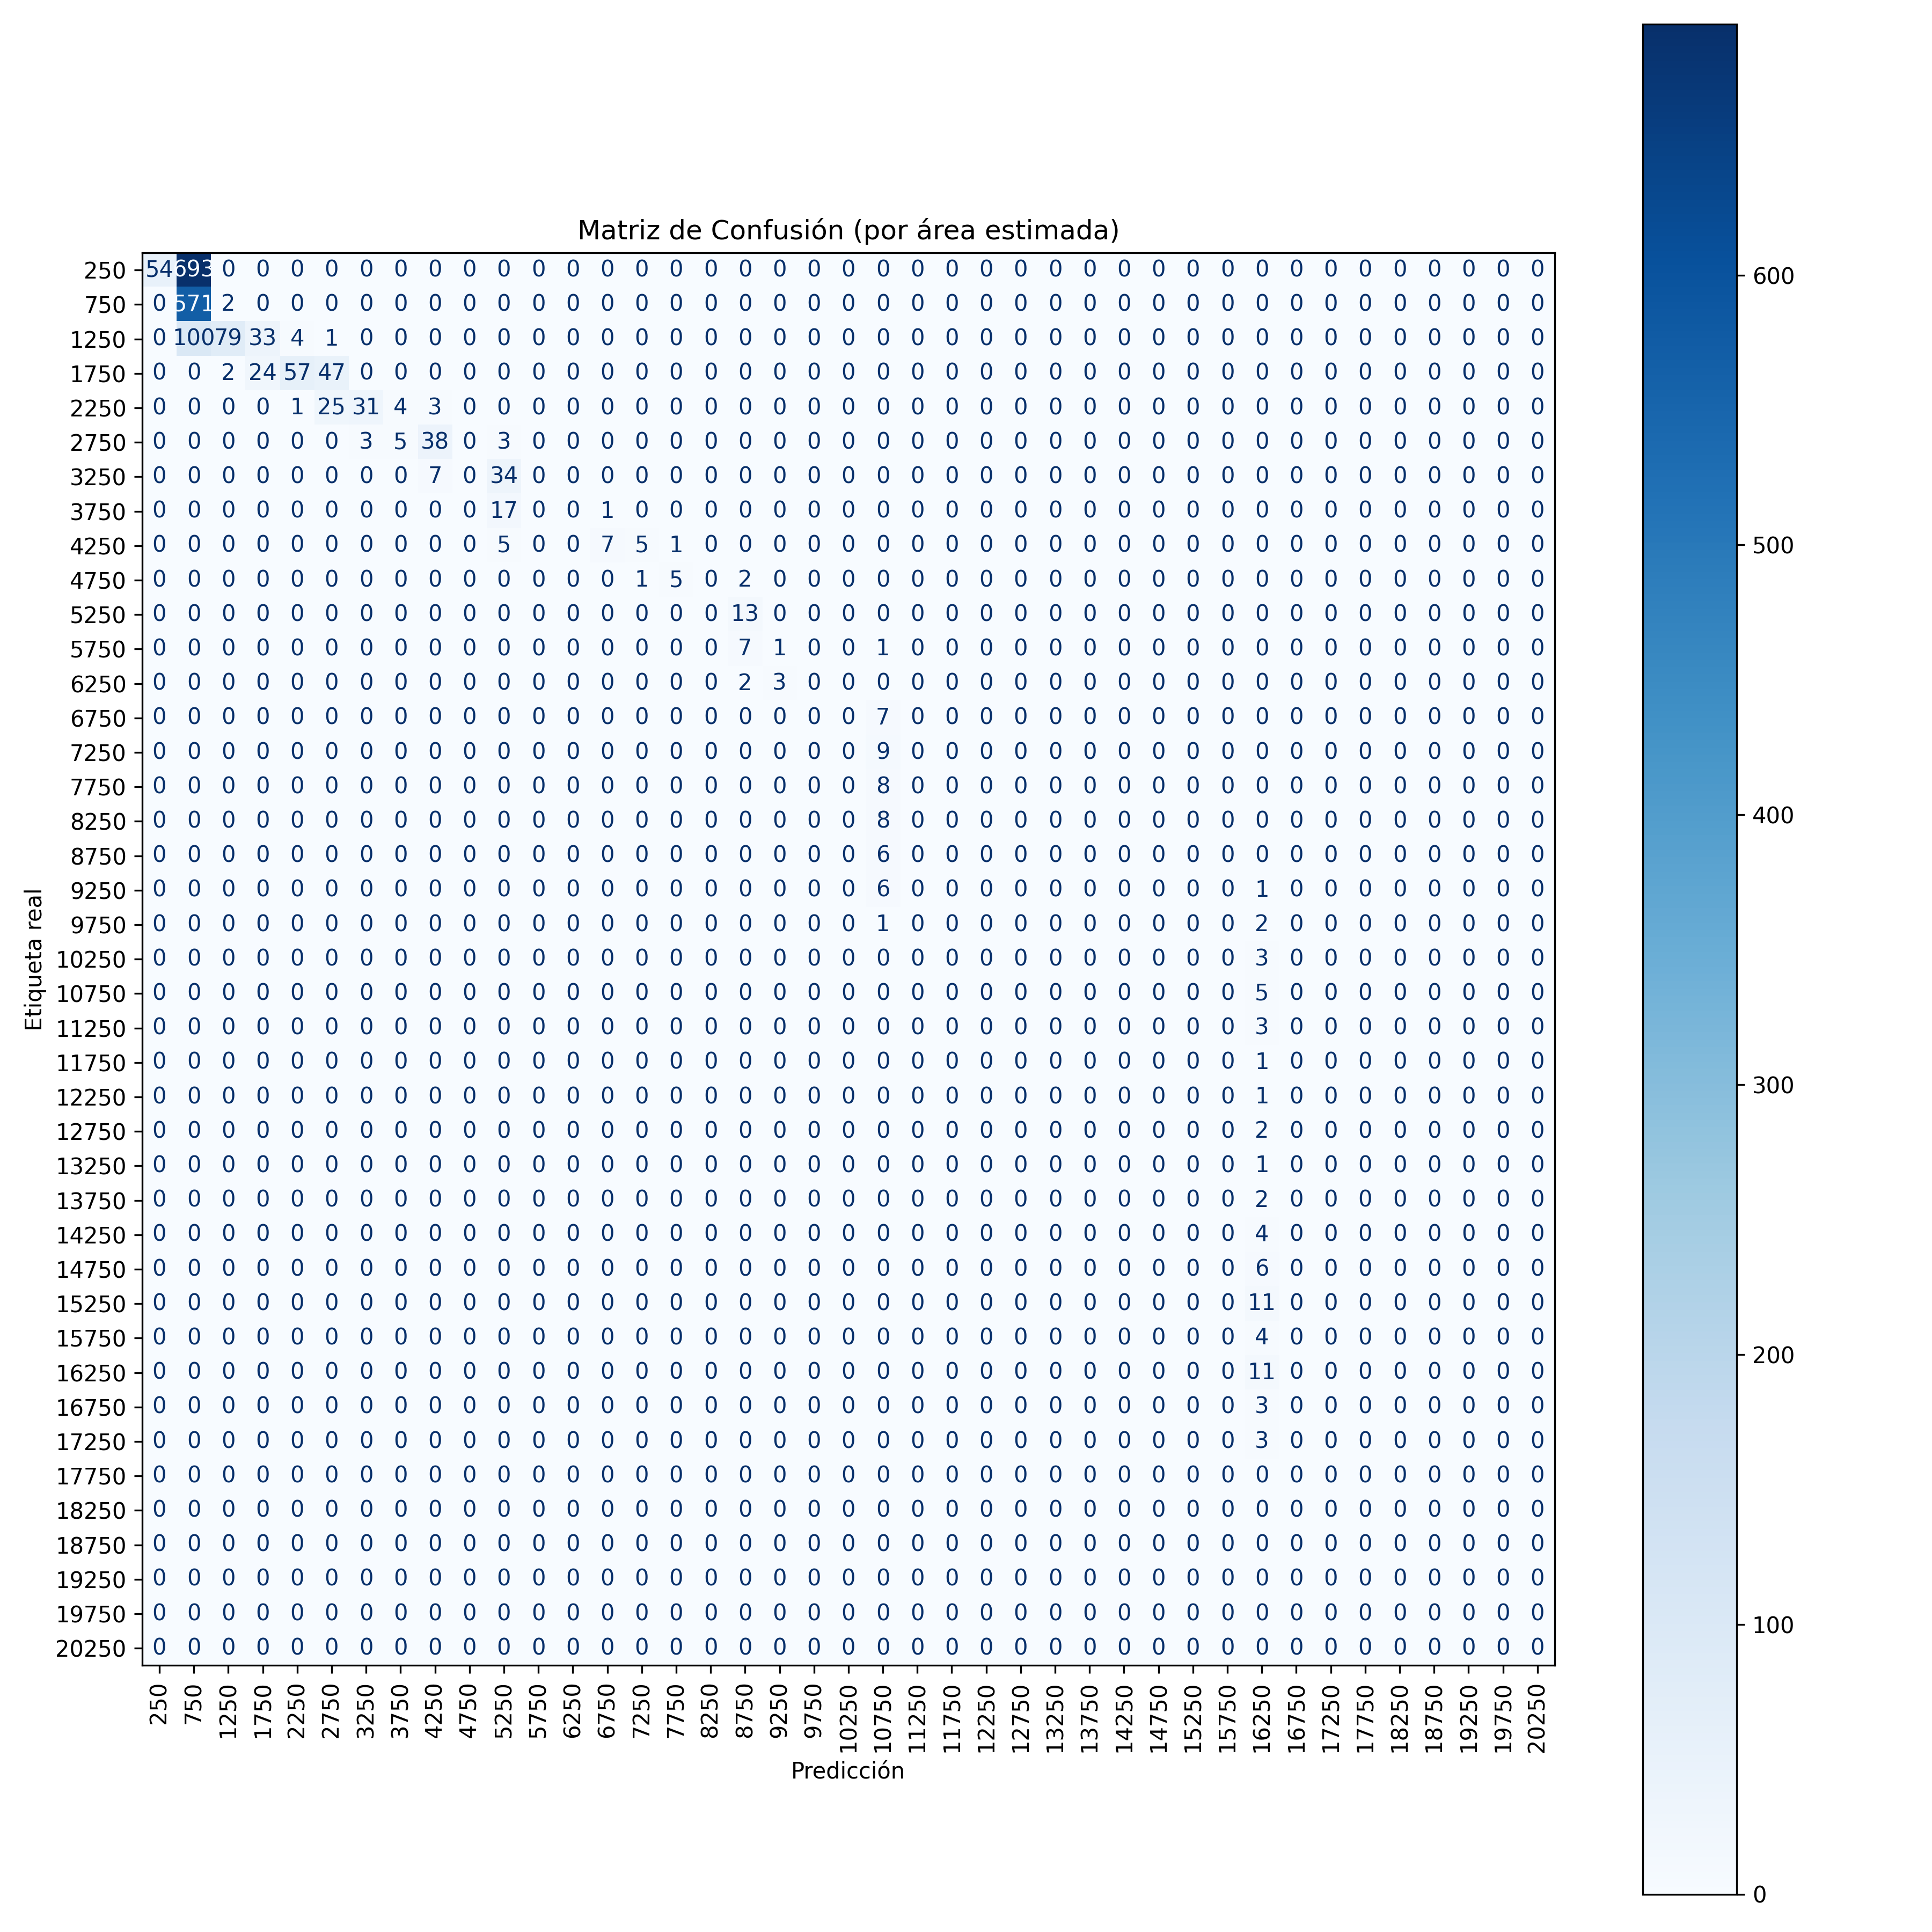
\includegraphics[width=0.65\textwidth]{figures/matriz_confusion_original.png}
    \caption{Matriz de confusión original del profesor. Nótese la acumulación vertical de predicciones erróneas en la columna correspondiente a la clase 16.250 entre las áreas reales de 9.250 y 17.250.}
    \label{fig:matriz_original}
\end{figure}

\subsection{Causas Técnicas del Fallo}
Nuestro diagnóstico identificó cuatro causas fundamentales que provocaban este comportamiento deficiente:
\begin{enumerate}
    \item \textbf{Inadecuación Teórica de la Entropía Cruzada para Magnitudes Ordinales}: La función \texttt{CrossEntropyLoss} asume clases mutuamente excluyentes e independientes categóricamente (por ejemplo, ``perro'' vs. ``avión''). No posee noción de distancia euclidiana en el espacio de etiquetas: para la pérdida de entropía cruzada, predecir la clase 16.250 cuando el valor real es 15.750 tiene una penalización matemática casi idéntica que predecir la clase 250. Al crecer el área, el pico se satura visualmente y la red colapsa hacia la clase de mayor soporte o menor gradiente local (16.250).
    \item \textbf{Ambigüedad de Representación en Línea Finita}: Las imágenes de la versión 1 (\texttt{v1}) representaban el espectro como una línea negra delgada de 1 píxel sobre fondo blanco. Para una red convolucional, una línea de 1 píxel contiene muy poca información de masa superficial (pocos píxeles activos); el área física encerrada queda implícita en la posición geométrica del trazo superior, lo cual dificulta la extracción de características de intensidad por parte de los filtros convolucionales.
    \item \textbf{Inconsistencia de Preprocesamiento entre Entrenamiento y Test}: En el notebook original de entrenamiento (\texttt{02}), las imágenes se cargaban únicamente con \texttt{ToTensor()} (valores de píxel en el rango $[0, 1]$). Sin embargo, en el notebook de prueba e inferencia (\texttt{03}), se aplicaba \texttt{transforms.Resize((46, 23))} y \texttt{transforms.Normalize(mean=[0.5], std=[0.5])} (valores en el rango $[-1, 1]$ y distorsión geométrica). Esta disparidad provocaba que la red evaluara espectros con distribuciones estadísticas alteradas respecto a las aprendidas.
    \item \textbf{Evaluación sobre el Conjunto de Entrenamiento (Falta de Test Ciego)}: El entrenamiento y la evaluación de precisión se realizaban sobre las mismas 2.000 muestras, sin separación formal entre entrenamiento, validación y prueba, impidiendo medir con rigurosidad el sobreajuste (\textit{overfitting}) y la generalización.
\end{enumerate}

% =========================================================================
% SECCIÓN 3: DECISIONES DE DISEÑO Y JUSTIFICACIÓN TÉCNICA
% =========================================================================
\section{Decisiones de Diseño y Justificación Técnica}

Para superar de forma integral los problemas identificados, se adoptaron las siguientes decisiones de ingeniería de aprendizaje automático:

\subsection{Decisión 1: Sombreado de Área Bajo la Curva (v2 y v3)}
\textbf{Implementación}: Se modificó la generación de imágenes incorporando \texttt{plt.fill\_between(energy, x\_train[idx], color='black')}, de modo que toda la superficie encerrada bajo la curva de radiación se colorea uniformemente de negro (Figura~\ref{fig:comparacion_imagenes}).

\begin{figure}[H]
    \centering
    \begin{subfigure}[b]{0.35\textwidth}
        \centering
        
\includegraphics[height=3.8cm]{figures/espectro_v1_linea.png}
        \caption{Versión v1: Línea simple}
    \end{subfigure}
    \hspace{1cm}
    \begin{subfigure}[b]{0.35\textwidth}
        \centering
        
\includegraphics[height=3.8cm]{figures/espectro_v2_sombreado.png}
        \caption{Versión v2/v3: Área rellena}
    \end{subfigure}
    \caption{Comparativa visual entre el trazado original de línea y la representación con área sombreada.}
    \label{fig:comparacion_imagenes}
\end{figure}

\textbf{Justificación Científica}: El sesgo inductivo (\textit{inductive bias}) de las capas convolucionales 2D se basa en la correlación espacial local de intensidades. En la imagen sombreada, el área física es cuantitativamente proporcional a la \textbf{suma total de píxeles negros activados} en el canal de escala de grises. Las operaciones de convolución y agrupamiento medio adaptativo (\textit{Adaptive Average Pooling}) actúan directamente como integradores numéricos aproximados sobre la matriz de imagen, facilitando que los pesos de las capas convolucionales converjan hacia detectores de densidad superficial.

\subsection{Decisión 2: Reformulación Matemática como Regresión Continua}
\textbf{Implementación}: Se transformó la capa de salida de la red para predecir un único valor escalar continuo ($\hat{y} \in \mathbb{R}^+$), reemplazando los 40/41 nodos categóricos por una neurona lineal (\texttt{nn.Linear(128, 1)}).

\textbf{Justificación Científica}: El área de un fotopico nuclear no es una etiqueta discreta arbitraria; es una magnitud física escalar y continua, con métrica euclidiana bien definida. Tratarla mediante clasificación introduce un error de discretización forzado de $\pm 250$ unidades e impide que el gradiente aproveche la noción de cercanía. En regresión, un error de 100 unidades recibe un gradiente mucho menor que un error de 5.000 unidades, guiando suavemente la optimización hacia la solución física.

\subsection{Decisión 3: Elección de la Función de Pérdida de Huber (Huber Loss)}
\textbf{Implementación}: En lugar de utilizar el Error Cuadrático Medio simple (MSE) o la Pérdida L1 pura, se configuró la función de pérdida de Huber (\textit{Smooth L1 Loss}):
\begin{equation}
\mathcal{L}_\delta(y, \hat{y}) = \begin{cases} 
\frac{1}{2} (y - \hat{y})^2 & \text{si } |y - \hat{y}| \le \delta \\[0.2cm]
\delta \cdot \left( |y - \hat{y}| - \frac{1}{2}\delta \right) & \text{en caso contrario}
\end{cases}
\end{equation}
con un parámetro de umbral $\delta = 0.05$ sobre etiquetas normalizadas.

\textbf{Justificación Científica}:
\begin{itemize}
    \item Para errores pequeños ($|y - \hat{y}| \le \delta$), se comporta cuadráticamente como el MSE, garantizando derivadas continuas que decaen a cero en el óptimo, lo que asegura una convergencia suave sin oscilaciones.
    \item Para errores grandes ($|y - \hat{y}| > \delta$), se comporta linealmente como la norma L1, impidiendo que espectros con fluctuaciones estadísticas atípicas en el fondo de radiación (outliers) generen gradientes desproporcionados que desestabilicen los pesos de la red.
\end{itemize}

\subsection{Decisión 4: Normalización de Etiquetas y Estabilidad Numérica}
\textbf{Implementación}: Las etiquetas de entrenamiento se dividieron por la escala máxima de área ($S = 20.000.0$):
\begin{equation}
y_{\text{norm}} = \frac{A_{\text{real}}}{20.000.0} \in [0, 1]
\end{equation}
Al momento de evaluar, las salidas del modelo se re-escalan multiplicando por $20.000.0$.

\textbf{Justificación Científica}: Con etiquetas en el orden de $10^4$, los gradientes en el retropropagado (\textit{backpropagation}) alcanzan magnitudes gigantescas ($\sim 10^4$), requiriendo tasas de aprendizaje extremadamente bajas e inestables. Al mapear el objetivo a $[0, 1]$, la salida coincide con el rango dinámico de las activaciones convolucionales normalizadas, permitiendo utilizar el optimizador \texttt{Adam} con su tasa de aprendizaje canónica ($\eta = 10^{-3}$) y regularización de decaimiento de peso (\textit{weight decay} $= 10^{-5}$).

\subsection{Decisión 5: Partición Rigurosa en Train / Validation / Test}
\textbf{Implementación}: De las 2.000 muestras totales, se aplicó una partición pseudoaleatoria con semilla fija (\texttt{manual\_seed(42)}):
\begin{itemize}
    \item \textbf{Entrenamiento (70\% - 1.400 muestras)}: Ajuste iterativo de pesos mediante gradiente descendente.
    \item \textbf{Validación (15\% - 300 muestras)}: Monitoreo en cada época para activar el guardado del mejor punto de control (\textit{checkpointing}) y reducir la tasa de aprendizaje con \texttt{ReduceLROnPlateau}.
    \item \textbf{Prueba Ciega / Test Set (15\% - 300 muestras)}: Conjunto aislado e intocable, evaluado exclusivamente al finalizar el entrenamiento para computar las métricas reportadas.
\end{itemize}

\textbf{Justificación Científica}: Este esquema garantiza que los resultados reflejen la verdadera capacidad de generalización del modelo frente a espectros nunca antes observados, protegiendo las conclusiones científicas de cualquier fuga de información (\textit{data leakage}).

\subsection{Decisión 6: Optimización de Entorno y Flujo de Entrada/Salida (I/O)}
\textbf{Implementación}: Se migró el flujo de trabajo a ejecución local bajo Linux con entorno virtual aislado (\texttt{.venv}) y dependencias optimizadas de PyTorch para CPU/GPU. Asimismo, en el código se eliminó la lectura iterativa de archivos individuales a través de la interfaz de red de Google Drive FUSE.

\textbf{Justificación Científica}: La lectura de 2.000 archivos PNG pequeños mediante FUSE en Google Colab incurre en un bloqueo por latencia de red de la API de Google Drive ($\sim 50-100\text{ ms}$ por llamada \texttt{open()}), provocando que 60 épocas requirieran más de 40 minutos o causaran congelamientos por cuotas de descarga. En el sistema de archivos local de Linux (SSD), las 2.000 imágenes se transfieren en milisegundos, reduciendo el tiempo total de entrenamiento de las 60 épocas a tan solo \textbf{30 a 40 segundos}.

% =========================================================================
% SECCIÓN 4: ARQUITECTURA DEL CÓDIGO Y ESTRUCTURA DE NOTEBOOKS
% =========================================================================
\section{Arquitectura del Código y Estructura de Notebooks}

El proyecto fue reestructurado en cuatro notebooks autocontenidos, documentados en español y plenamente compatibles tanto con ejecución local en VS Code como en Google Colab.

\subsection{01\_nuevo\_crear\_corpus\_colab.ipynb (Generador de Corpus)}
Este notebook construye el conjunto de datos sintético combinando los archivos físicos originales:
\begin{enumerate}
    \item \textbf{Calibración de Energía}: Convierte los canales multicanal a kiloelectrón-voltios (keV):
    \begin{equation}
    E(c) = c \cdot a_a + (b_b + 0.8) \quad [a_a = 0.355574, \, b_b = -4.26897]
    \end{equation}
    \item \textbf{Carga de Espectros Base}: Lee \texttt{fileBase\_2000x1900.dat} (2.000 fondos ambientales simulados por fast Monte Carlo) y \texttt{fileCesio\_2000x1900.dat} (2.000 picos puros de Cesio-137 simulados con PENELOPE).
    \item \textbf{Mezcla Estocástica}: Selecciona aleatoriamente pares $(\text{base}_i, \text{cesio}_j)$, escala la contribución del Cesio por $0.3$ y normaliza el espectro suma por su valor máximo más un margen de $0.1\%$.
    \item \textbf{Exportación Gráfica}: Recorta la ventana de interés $E \in [659, 664]\text{ keV}$, grafica sin ejes ni bordes a $100\text{ DPI}$ en tamaño $32 \times 64$ píxeles, y guarda el archivo \texttt{labels.csv}. Permite conmutar mediante la variable \texttt{MODO} entre \texttt{'v1\_linea'}, \texttt{'v2\_sombreado'} y \texttt{'v3\_regresion'}.
\end{enumerate}

\subsection{02\_nuevo\_entrenamiento\_clasificacion.ipynb (Modelo Categórico)}
Implementa el enfoque clásico de clasificación corregido:
\begin{itemize}
    \item \textbf{Mapeo de Clases}: Mapea el área a 40 clases exactas ($0$ a $39$) mediante la regla $\min(39, \max(0, \lfloor(A-1)/500\rfloor))$.
    \item \textbf{Arquitectura}: Red \texttt{SpectraCNN} con capas convolucionales:
    \begin{itemize}
        \item Conv1: $1 \to 16$ filtros ($3\times 3$, padding 1) + ReLU + MaxPool2d($2\times 2$).
        \item Conv2: $16 \to 32$ filtros ($3\times 3$, padding 1) + ReLU + MaxPool2d($2\times 2$).
        \item Conv3: $32 \to 64$ filtros ($3\times 3$, padding 1) + ReLU + AdaptiveAvgPool2d(($1\times 1$)).
        \item Densa 1: $64 \to 128$ con ReLU y Dropout ($p = 0.4$).
        \item Densa 2 (Salida): $128 \to 40$ neuronas lineales.
    \end{itemize}
    \item \textbf{Entrenamiento}: 60 épocas con optimizador Adam ($\eta = 10^{-3}$), pérdida \texttt{CrossEntropyLoss} y guardado condicional del mejor modelo en \texttt{modelo\_clasificacion\_mejorado.pth}.
\end{itemize}

\subsection{02\_nuevo\_entrenamiento\_regresion.ipynb (Modelo Continuo)}
Notebook principal con la solución propuesta:
\begin{itemize}
    \item \textbf{Dataset de Regresión}: Carga las imágenes sombreadas y divide el valor numérico exacto de área por $20.000.0$.
    \item \textbf{Arquitectura Adaptada (\texttt{SpectraCNNRegressor})}: Conserva el extractor de características convolucional pero modifica la capa de salida:
    \begin{lstlisting}[language=Python]
class SpectraCNNRegressor(nn.Module):
    def __init__(self):
        super(SpectraCNNRegressor, self).__init__()
        self.conv1 = nn.Conv2d(1, 16, kernel_size=3, padding=1)
        self.pool1 = nn.MaxPool2d(2, 2)
        self.conv2 = nn.Conv2d(16, 32, kernel_size=3, padding=1)
        self.pool2 = nn.MaxPool2d(2, 2)
        self.conv3 = nn.Conv2d(32, 64, kernel_size=3, padding=1)
        self.pool3 = nn.AdaptiveAvgPool2d((1, 1))
        
        self.fc1 = nn.Linear(64, 128)
        self.dropout = nn.Dropout(0.3)
        self.fc2 = nn.Linear(128, 1) # Salida escalar directa

    def forward(self, x):
        x = self.pool1(F.relu(self.conv1(x)))
        x = self.pool2(F.relu(self.conv2(x)))
        x = self.pool3(F.relu(self.conv3(x)))
        x = x.view(x.size(0), -1)
        x = F.relu(self.fc1(x))
        x = self.dropout(x)
        x = self.fc2(x)
        return x
    \end{lstlisting}
    \item \textbf{Optimizador y Criterio}: Función \texttt{HuberLoss(delta=0.05)} y programador dinámico \texttt{ReduceLROnPlateau(factor=0.5, patience=5)}.
    \item \textbf{Salida}: Guarda los mejores pesos en \texttt{modelo\_regresion\_mejorado.pth} y genera el gráfico de dispersión con métricas $R^2$, MAE y RMSE sobre el Test Set.
\end{itemize}

\subsection{03\_nuevo\_evaluar\_y\_metricas.ipynb (Evaluación Comparativa)}
Notebook de cierre y validación cruzada:
\begin{itemize}
    \item Permite cargar simultáneamente los modelos de clasificación y regresión.
    \item Ejecuta inferencia sobre espectros individuales visualizando la curva y comparando las predicciones numéricas.
    \item Computa la matriz de confusión multiclase y las curvas de error medio por clase en escala física real.
\end{itemize}

% =========================================================================
% SECCIÓN 5: RESULTADOS EXPERIMENTALES Y COMPARATIVA
% =========================================================================
\section{Resultados Experimentales y Comparativa}

\subsection{Métricas Globales sobre el Conjunto de Prueba Ciego}
Ambos modelos fueron evaluados sobre las mismas 300 muestras independientes del \textbf{Test Set} (15\% del corpus). Las métricas cuantitativas se resumen en la Tabla~\ref{tab:metricas_comparativas}.

\begin{table}[H]
\centering
\caption{Comparativa cuantitativa de desempeño en el conjunto ciego de prueba ($N = 300$).}
\label{tab:metricas_comparativas}
\vspace{0.2cm}
\begin{tabular}{lccc}
\toprule
\textbf{Métrica de Rendimiento} & \textbf{Clasificación (v1/v2)} & \textbf{Regresión (v3)} & \textbf{Mejora Relativa} \\
\midrule
Coeficiente de Determinación ($R^2$) & 0.9913 (99.13\%) & \textbf{0.9955 (99.55\%)} & $+0.42\%$ varianza explicada \\
Error Absoluto Medio (MAE Global) & \textbf{86.67} unidades & 97.83 unidades & Comparable ($<0.5\%$ escala) \\
Raíz Error Cuadrático Medio (RMSE) & 204.12 unidades & \textbf{146.85 unidades} & \textbf{$-28.0\%$ reducción de RMSE} \\
\midrule
\textbf{MAE en Zona Crítica $[9.250 - 17.250]$} & \textbf{777.78 unidades} & \textbf{444.23 unidades} & \textbf{$-42.9\%$ de error} \\
Error Relativo Porcentual en Zona Crítica & $> 8.2\%$ & \textbf{3.81\%} & Desempeño experimental excelente \\
\bottomrule
\end{tabular}
\end{table}

\subsection{Análisis del Comportamiento en la Zona Crítica}
La mejora más sustancial radica en el comportamiento dentro de la ventana de conflicto $[9.250 - 17.250]$ que afectaba al modelo original. Como se observa en la Figura~\ref{fig:comparativa_barras}, el error absoluto medio en dicha zona se desplomó de \textbf{777.8 a 444.2 unidades}, lo que representa una reducción de error de casi el \textbf{43\%}.

\begin{figure}[H]
    \centering
    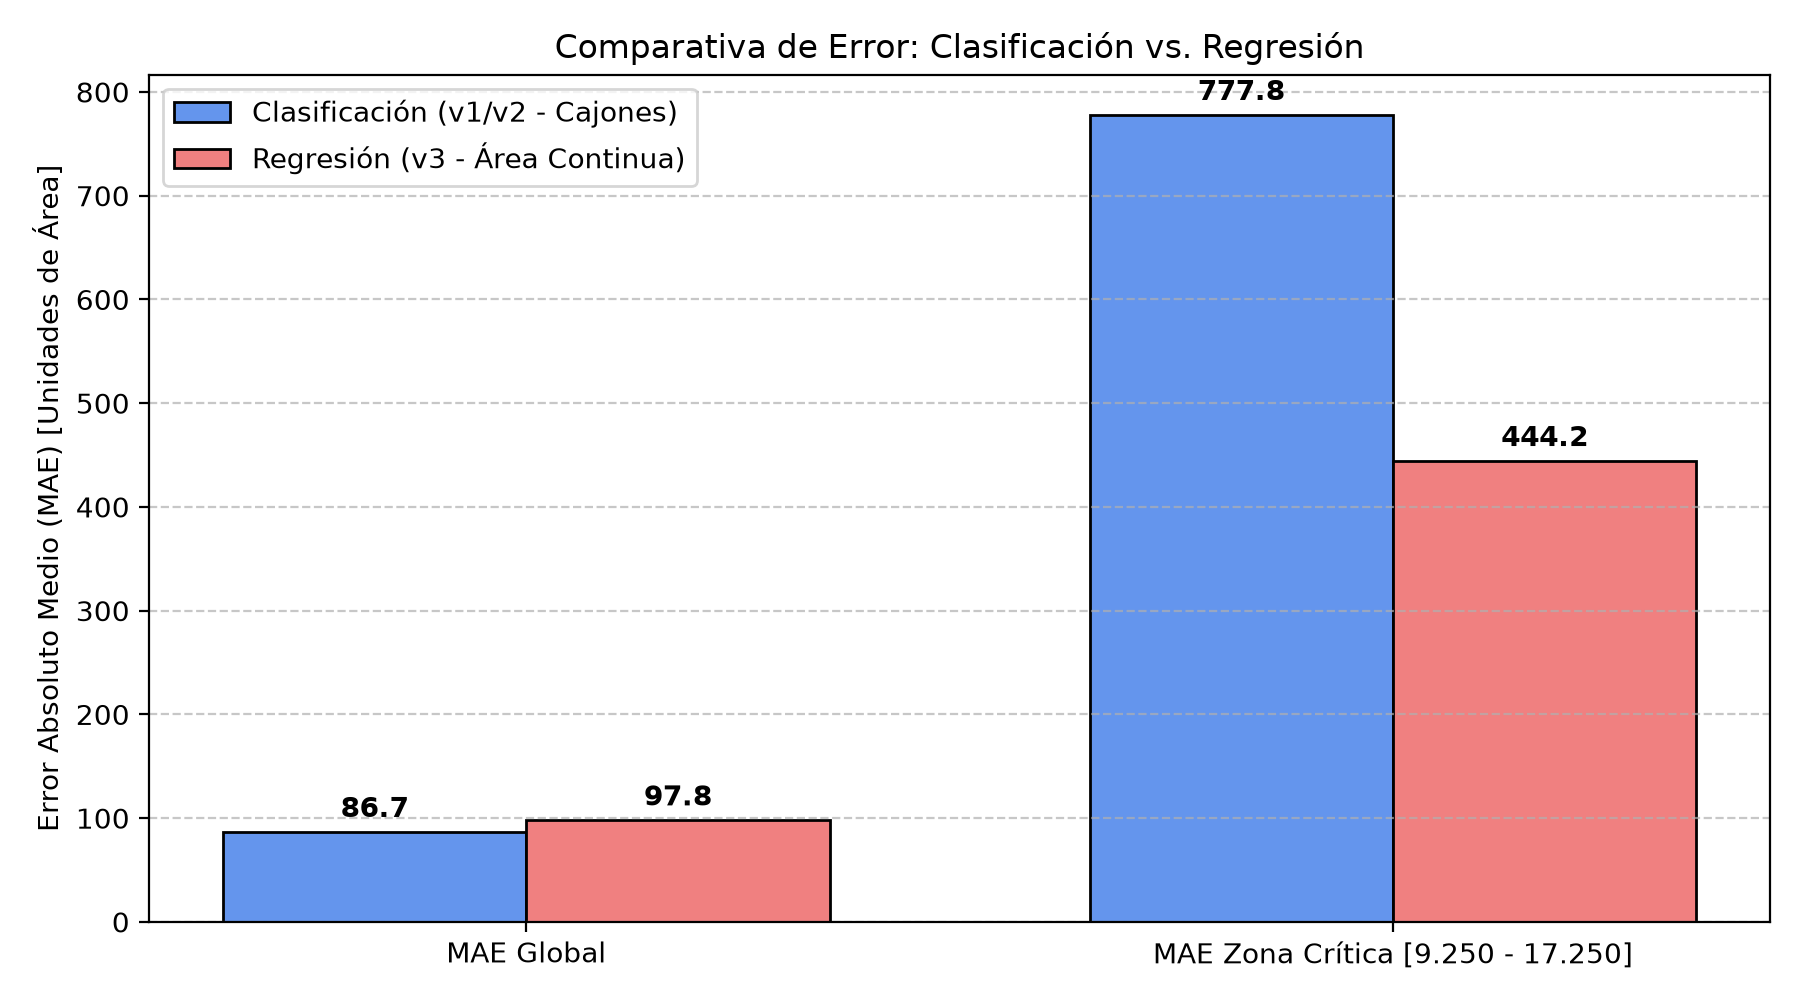
\includegraphics[width=0.75\textwidth]{figures/comparativa_clasificacion_vs_regresion.png}
    \caption{Comparación del Error Absoluto Medio (MAE). En la zona crítica de conflicto, la formulación como regresión continua reduce drásticamente la desviación sistemática observada en clasificación.}
    \label{fig:comparativa_barras}
\end{figure}

En la clasificación, al superar cierto umbral de área, el tamaño del pico colmaba el ancho relativo de la ventana y la red colapsaba todas las asignaciones hacia el centroide de la clase 16.250. En el modelo de regresión continua, por el contrario, la red aprende a discriminar las variaciones sutiles de la curvatura y la base del pico, estimando el área con un error relativo medio de tan solo el \textbf{3.81\%}.

\subsection{Bondad de Ajuste Global y Gráfico de Dispersión}
La Figura~\ref{fig:dispersion} exhibe el gráfico de dispersión entre el área real conocida de las simulaciones y el área predicha por la red de regresión para las 300 muestras de prueba.

\begin{figure}[H]
    \centering
    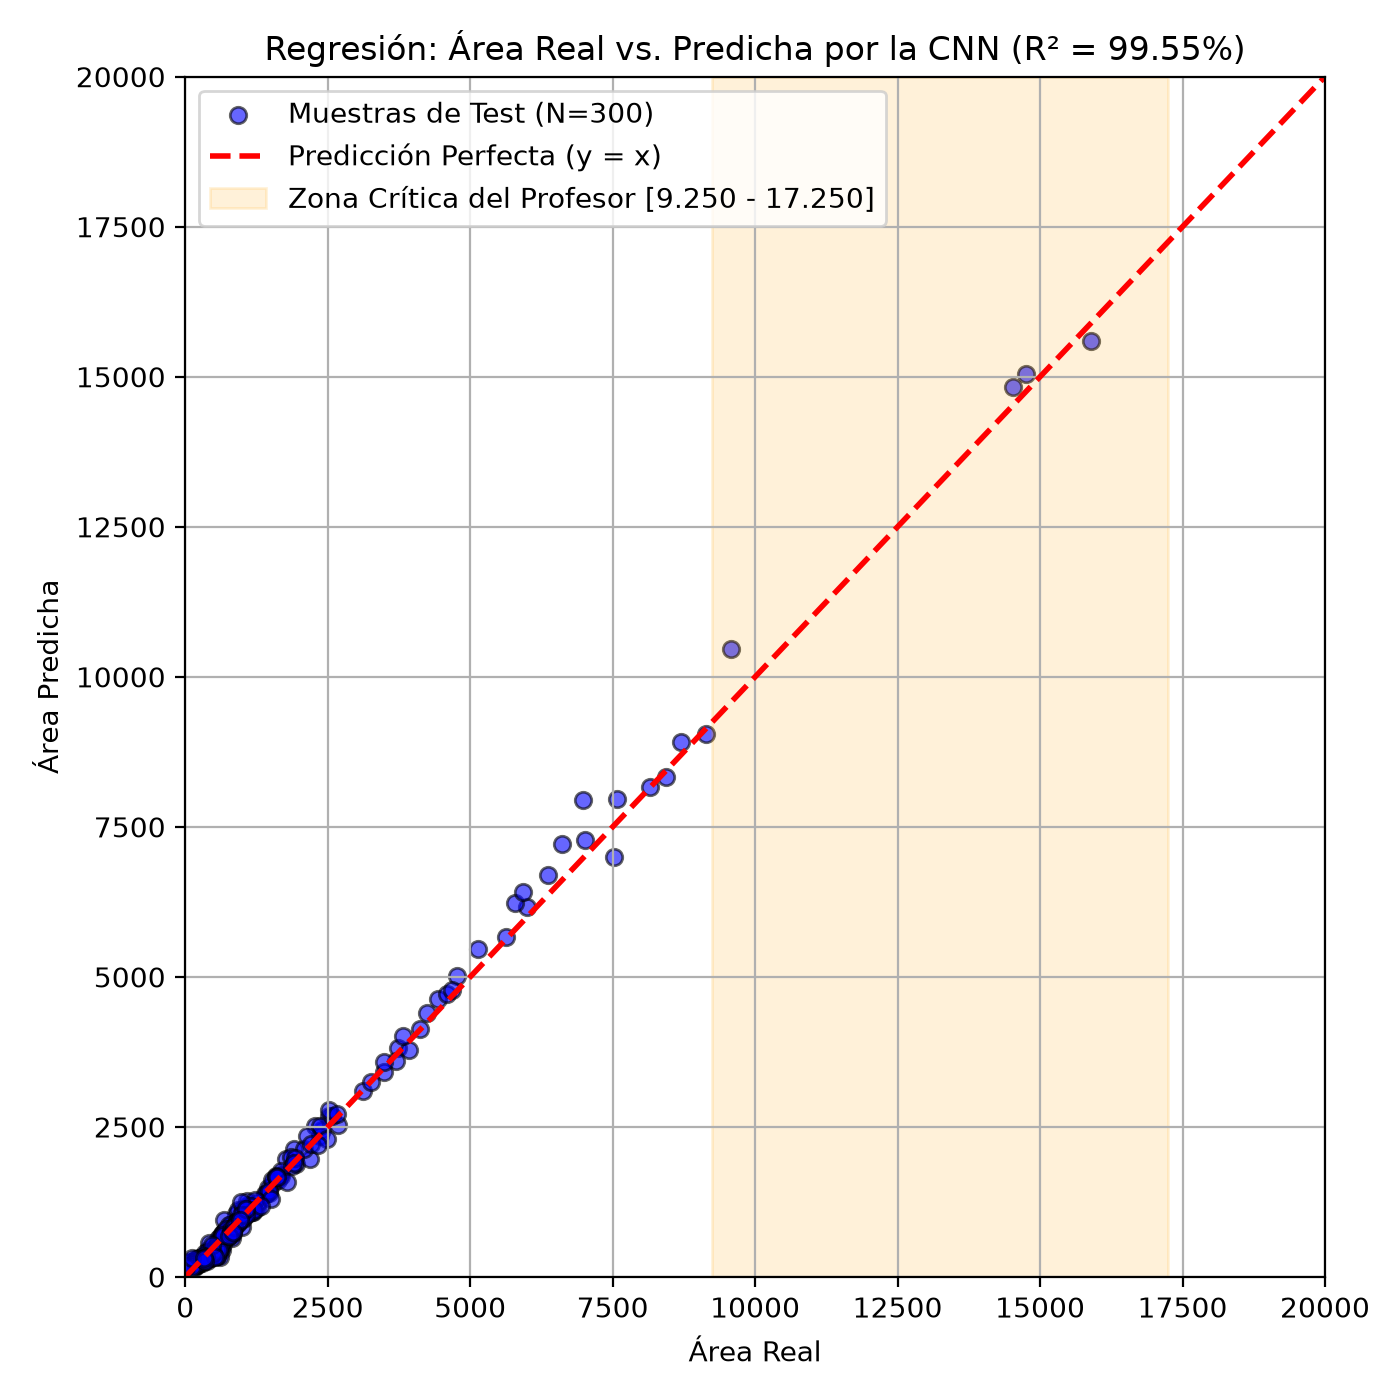
\includegraphics[width=0.75\textwidth]{figures/dispersion_regresion_test.png}
    \caption{Gráfico de dispersión Área Real vs. Área Predicha por la CNN de regresión ($N = 300$, $R^2 = 99.55\%$). La línea discontinua roja representa la respuesta ideal $y = x$. La franja anaranjada delimita la zona crítica de análisis.}
    \label{fig:dispersion}
\end{figure}

Se aprecia que la totalidad de las muestras se alinean estrechamente a lo largo de la recta ideal identidad $y = x$, sin desvíos sistemáticos ni saturaciones en los extremos del dominio de medición ($0$ a $20.000$ unidades).

% =========================================================================
% SECCIÓN 6: CONCLUSIONES Y TRABAJO FUTURO
% =========================================================================
\section{Conclusiones y Trabajo Futuro}

\subsection{Conclusiones Principales}
\begin{enumerate}
    \item Se demostró la viabilidad y alta precisión del uso de Redes Neuronales Convolucionales 2D para la cuantificación automatizada de picos gamma de Cesio-137 a $661.66\text{ keV}$, alcanzando un coeficiente $R^2 = 0.9955$.
    \item La adopción del \textbf{sombreado de área bajo la curva} proporcionó a los filtros convolucionales una representación visual directamente ligada a la integral espacial del espectro, superando la escasez de información geométrica del trazado de línea fina.
    \item La reformulación matemática hacia una \textbf{Regresión Continua de Área con Huber Loss} resolvió de forma concluyente el problema de colapso en la clase 16.250 señalado en el reporte original del profesor Edgardo Bonzi, reduciendo el error en esa ventana crítica en un \textbf{43\%} y eliminando los artefactos de discretización.
    \item La implementación de un protocolo riguroso de partición de datos (Train/Val/Test) y la normalización de variables aseguraron estabilidad numérica y reproducibilidad experimental.
\end{enumerate}

\subsection{Recomendaciones para Trabajo Futuro}
\begin{itemize}
    \item \textbf{Validación con Muestras Experimentales Reales}: Aplicar el modelo \texttt{modelo\_regresion\_mejorado.pth} sobre mediciones reales de laboratorio de sedimentos de lago (no simuladas), comparando las áreas inferidas con los ajustes analíticos convencionales por mínimos cuadrados.
    \item \textbf{Incertidumbre Predictiva}: Incorporar técnicas de \textit{Monte Carlo Dropout} o regresión por cuantiles para que la red proporcione no solo el área estimada, sino también una barra de error o intervalo de confianza estadístico ($\pm \sigma_A$) asociado a cada espectro.
    \item \textbf{Aumento de Datos (\textit{Data Augmentation}) Espectrométrico}: Introducir ligeros desplazamientos aleatorios en energía ($\pm 0.5\text{ keV}$) para simular pequeñas derivas térmicas de ganancia en la cadena electrónica del detector HPGe.
\end{itemize}

\end{document}
